
\begin{frame}{$\chi_b$ yields in $\chi_b \to \TwoS$ decays}
  \setlength{\unitlength}{1mm}
  \centering
  \scalebox{0.7}{
  \begin{picture}(150,60)
    \put(0,0){
      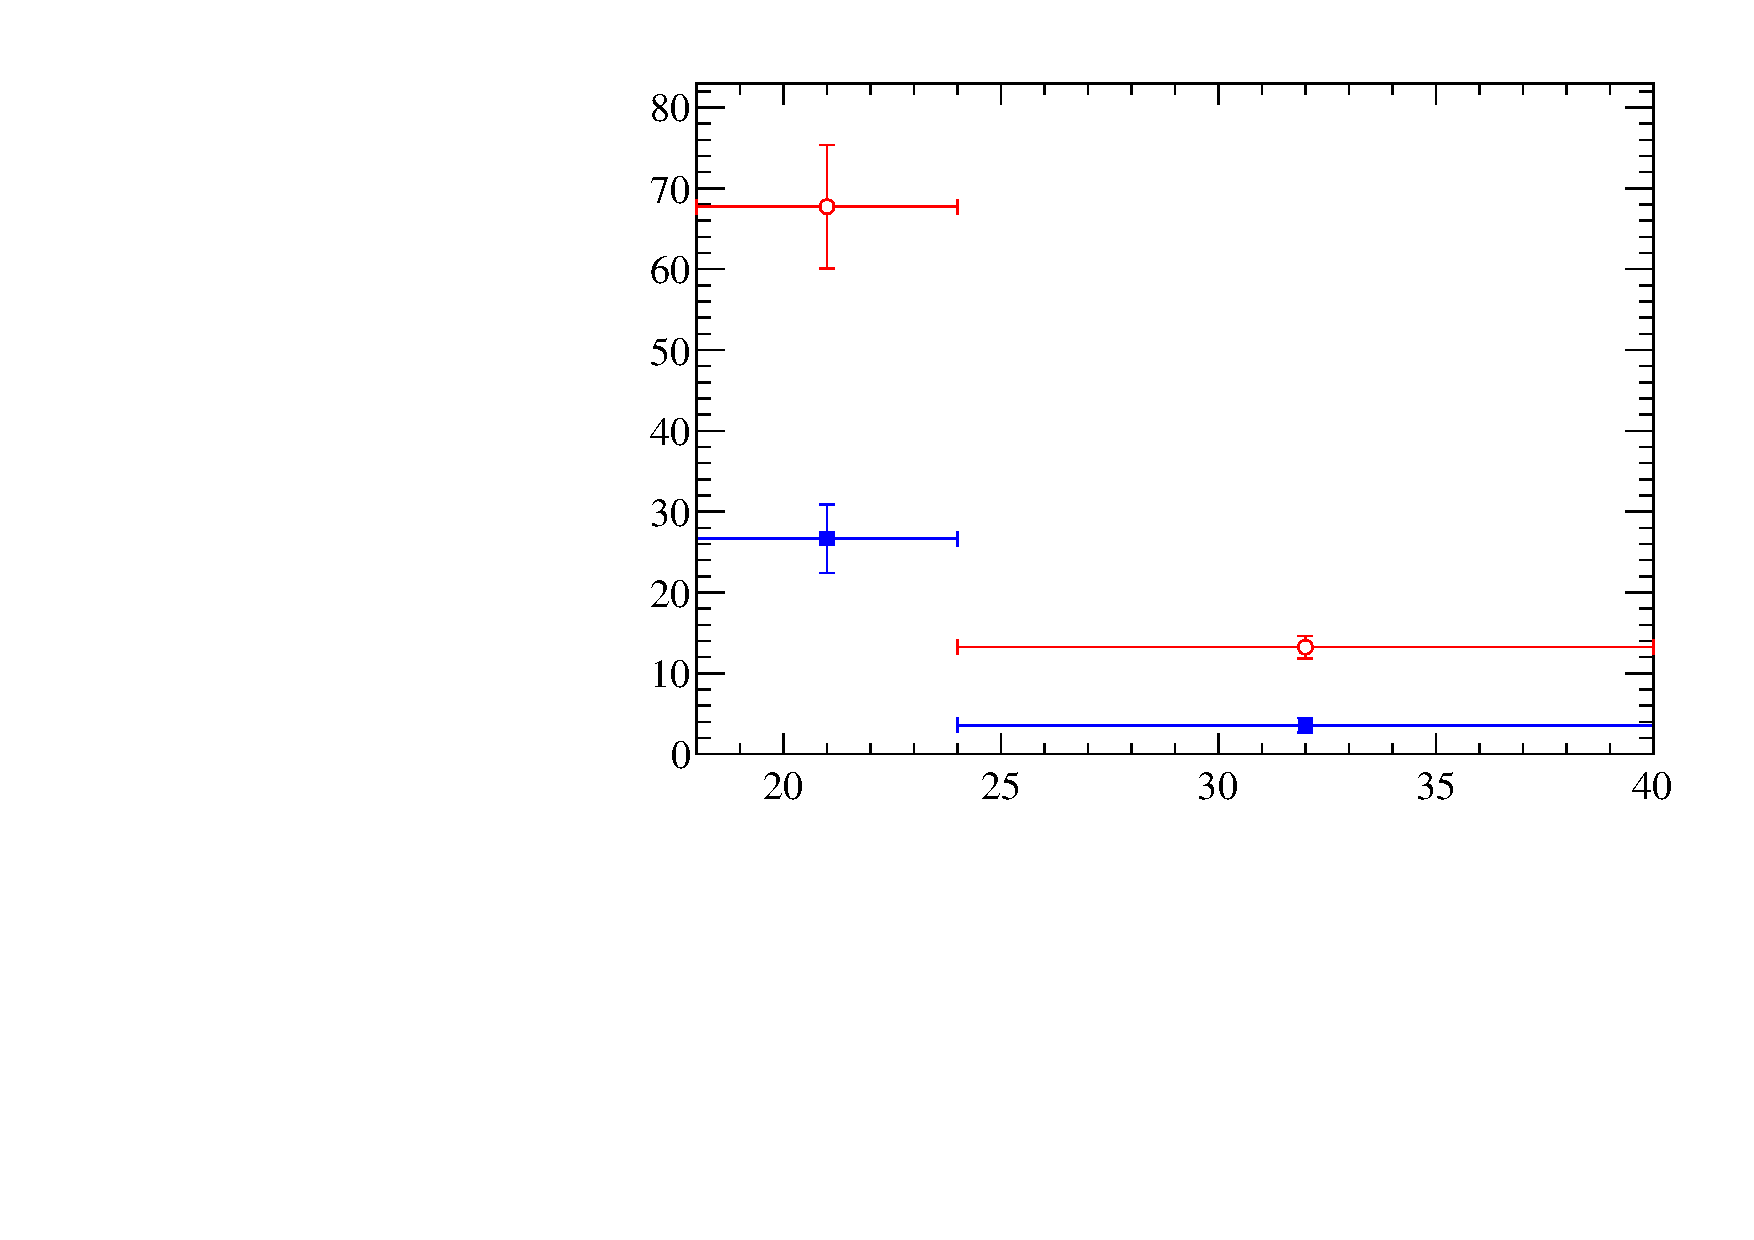
\includegraphics[width=75mm, height=60mm]{chib2s-yields/yields_2p}
    }
    \put(75,0){
      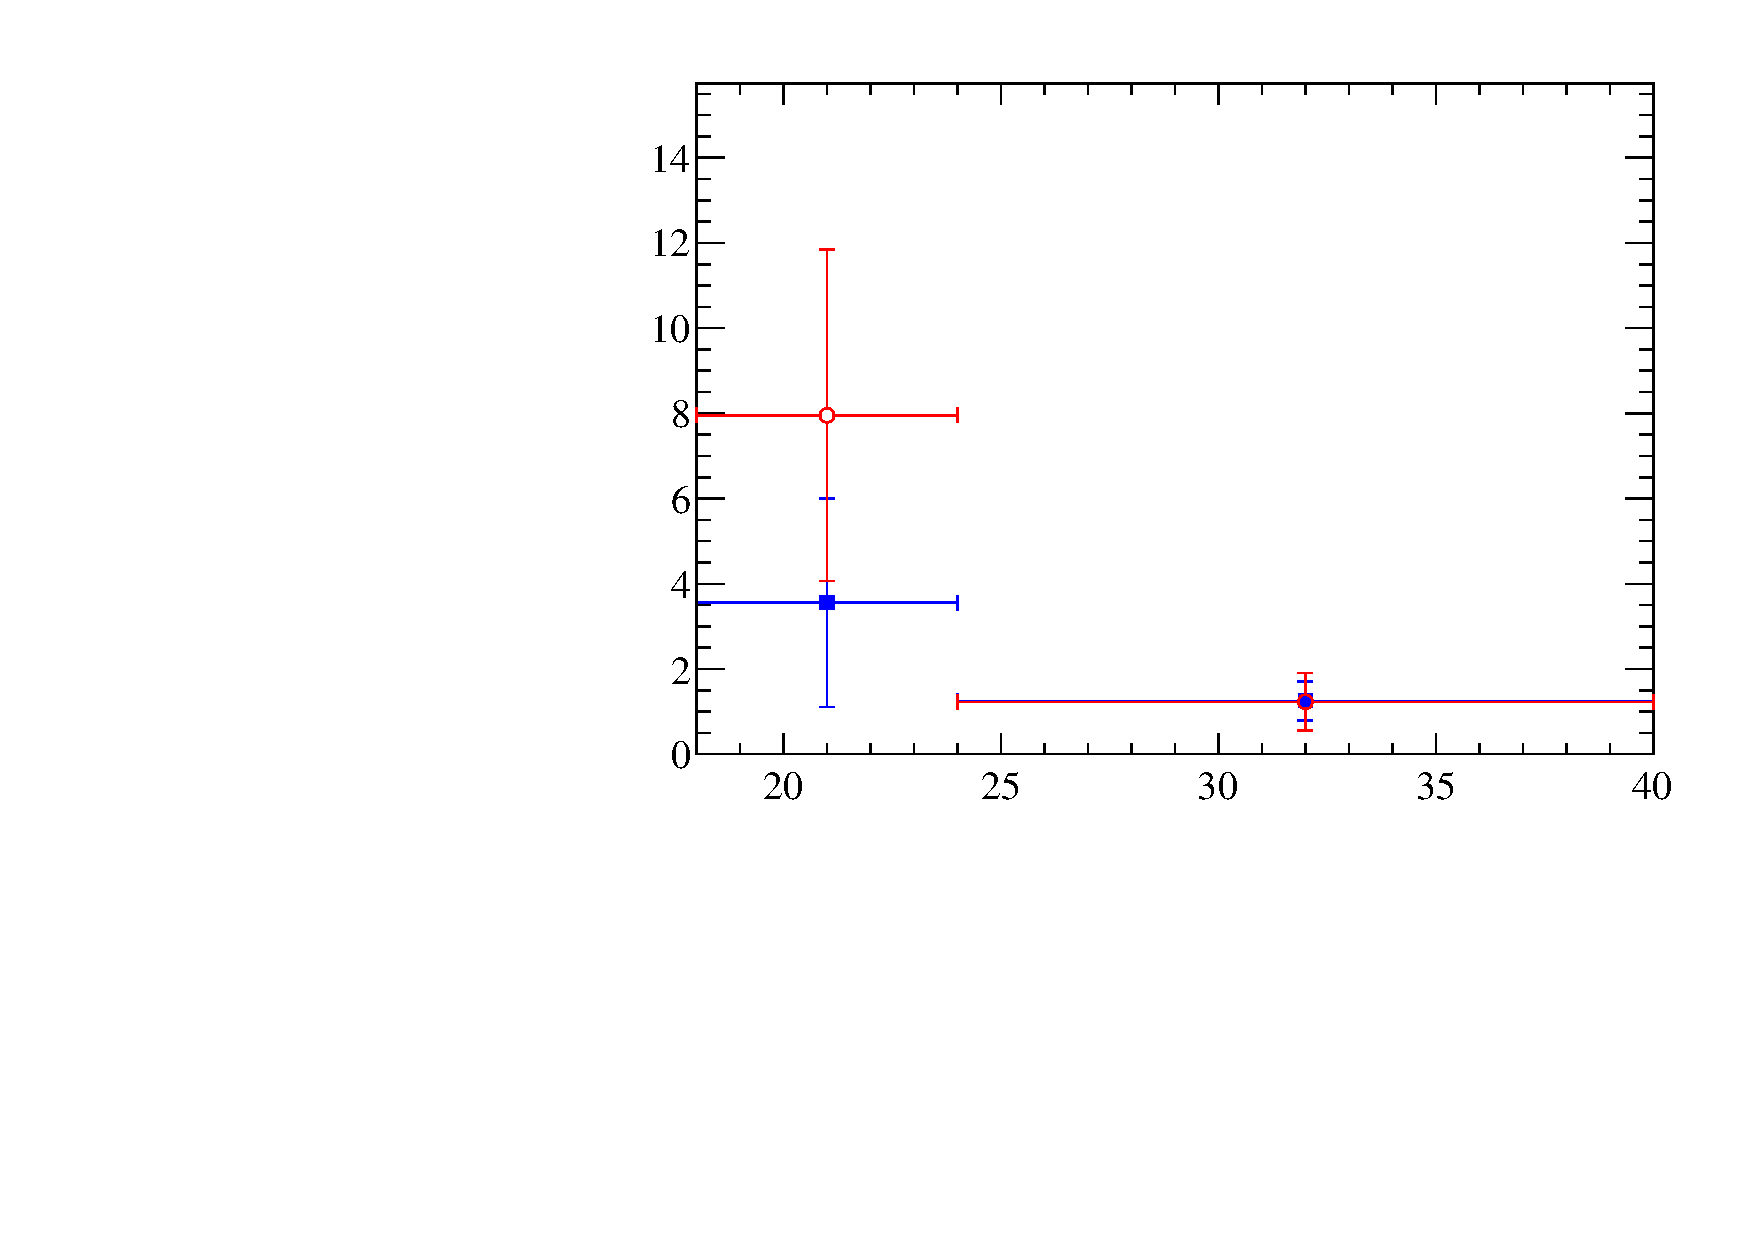
\includegraphics[width=75mm, height=60mm]{chib2s-yields/yields_3p}
    }


    \put(2,25){\begin{sideways}Events\end{sideways}}
    \put(35,2){$p_T^{\Y2S} \left[\gevc\right]$}
    \put(55,50){$\chibTwoP$}

    \put(77,25){\begin{sideways}Events\end{sideways}}
    \put(110,2){$p_T^{\Y2S} \left[\gevc\right]$}
    \put(130,50){$\chibThreeP$}


    \put(50,45){\textcolor{blue}{\sqs=7\tev}}
    \put(50,40){\textcolor{red}{\sqs=8\tev}}
    \put(45,45){
      
\includegraphics[width=3mm, height=2mm]{bsf}
    }
    \put(45,40){
      
\includegraphics[width=3mm, height=2mm]{rco}
    }

    \put(125,45){\textcolor{blue}{\sqs=7\tev}}
    \put(125,40){\textcolor{red}{\sqs=8\tev}}
    \put(120,45){
      
\includegraphics[width=3mm, height=2mm]{bsf}
    }
    \put(120,40){
      
\includegraphics[width=3mm, height=2mm]{rco}
    }

  % \graphpaper[5](0,0)(75, 60)
  \end{picture}
}
\begin{center}
Yields normilized by bin width.
\end{center}
\end{frame}

